\documentclass{article}%
\usepackage[T1]{fontenc}%
\usepackage[utf8]{inputenc}%
\usepackage{lmodern}%
\usepackage{textcomp}%
\usepackage{lastpage}%
\usepackage[head=40pt,margin=0.5in,bottom=0.6in]{geometry}%
\usepackage{graphicx}%
%
\title{\textbf{Ritmo y color en Carnaval de Tenerife}}%
\author{CLAUDIA HERNÁNDEZ}%
\date{04/03/2019}%
%
\begin{document}%
\normalsize%
\maketitle%
\textbf{URL: }%
http://www.eluniversal.com/guia{-}turistica/34712/ritmo{-}y{-}color{-}en{-}carnaval{-}de{-}tenerife\newline%
%
\textbf{Periodico: }%
EU, %
ID: %
34712, %
Seccion: %
guia{-}turistica\newline%
%
\textbf{Palabras Claves: }%
NO\_TIENE\newline%
%
\textbf{Derecho: }%
2.1%
, Otros Derechos: %
\newline%
%
\textbf{\textit{Multitud de personas se acercan todos los años a vivir esta fiesta, en la que no existen límites y sólo hay una obligación: divertirse.}}%
\newline%
\newline%
%
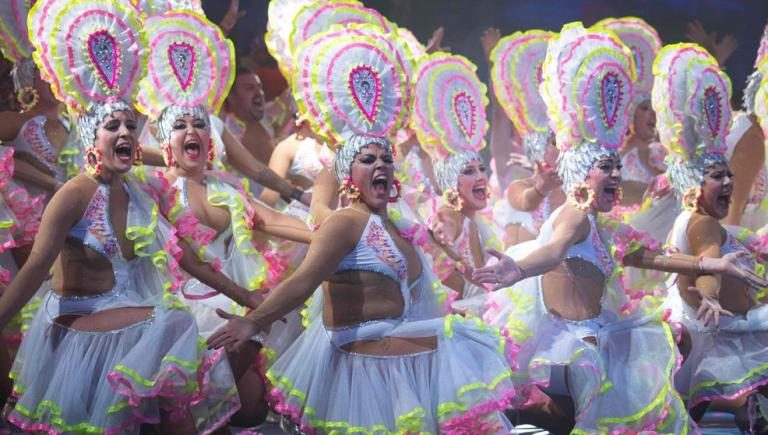
\includegraphics[width=300px]{EU_34712.jpg}%
\newline%
%
Multitud de personas se acercan todos los años a vivir esta fiesta, en la que no existen límites y sólo hay una obligación: divertirse.%
\newline%
%
Ritmo, color, desparpajo, lujo y, por supuesto, mucho espectáculo viven miles de personas en Tenerife.%
\newline%
%
El Carnaval de Santa Cruz de Tenerife es el más “brasileño” de todos los celebrados en España y es famoso internacionalmente por ser uno de los más populares del mundo.%
\newline%
%
Durante quince días la alegría, la libertad y la imaginación desbordan las calles de esta ciudad canaria.%
\newline%
%
Uno de los platos fuertes es la Gala de Elección de la Reina de las fiestas, que se suele celebrar el miércoles durante la primera semana de festejos. En este espectacular concurso, las candidatas derrochan glamour al desfilar sobre un escenario de 1.200 metros cuadrados, portando grandiosos trajes de increíbles fantasías que llegan a pesar más de cien kilos.%
\newline%
%
Tras ser elegida la reina, el viernes tiene lugar la Cabalgata anunciadora del Carnaval: miles de personas y decenas de agrupaciones musicales recorren durante horas las calles, formando una indescriptible serpiente multicolor de júbilo y descaro.%
\newline%
%
Durante los tres días siguientes, la música y las ganas de divertirse se adueñan de la ciudad, mientras actúan los distintos conjuntos carnavaleros que, a través de las letras de sus canciones llenas de ingenio e ironía, reflejan la realidad social y política con mucho sentido del humor.%
\newline%
%
Y cuando llega el martes de Carnaval se produce el colofón: el desfile del Coso, una gran cabalgata que sorprende a todo aquel que la presencia. Al día siguiente, el Entierro de la Sardina anuncia el fin de fiesta: el espíritu del Carnaval, representado por la sardina, se pasea por las calles en una carroza, para terminar ardiendo en llamas ante el desconsuelo de la “llorosa” corte de viudas, viudos y plañideras que la acompañan.%
\newline%
%
Sin embargo, la despedida definitiva será la celebración de la Piñata Chica durante el fin de semana, con actuaciones, verbenas y desfiles. Si decide venir a conocer el Carnaval de Santa Cruz de Tenerife, es conveniente que realice los preparativos con bastante antelación, ya que la demanda de este destino, de por sí uno de los más solicitados por su privilegiada situación que permite disfrutar del sol y la playa durante todo el año, aumenta en estas fechas.%
\newline%
%
Fuente: Turismo España%
\newline%
%
\end{document}